\documentclass[conference]{IEEEtran}

\usepackage[nocompress]{cite}
\usepackage{graphicx}
\usepackage{geometry}
\usepackage{pdflscape}
\usepackage{amsmath}
\usepackage{url}
\usepackage{pgfgantt}
\usepackage{ragged2e}
\usepackage{caption}
\usepackage{verbatim}

\begin{document}
\newgeometry{vmargin=2.25cm, hmargin=2.25cm}
\title{Translating SNAP Algorithm from OpenMP to CUDA}

\author{\IEEEauthorblockN{Andrew Lamzed-Short}
\IEEEauthorblockA{ID: 1897268}}

\maketitle

%%%%%%%%%%%%%%%%%%%%%%%%%%%%%%%%%%%%%%%%%%

\begin{abstract}

Mini-applications (``miniapps'') are small-scale, representative versions of large-scale pieces of scientific or engineering-focused software that seek to model the performance of an algorithm or program without actually executing the larger program. In this interim report, it is sought to examine the effects of altering the codebase of one such miniapp called ``SNAP'' from utilising only traditional processing cores to utilising a combination of computational processing cores and graphical processing cores and capabilities (mainly the latter), ultimately examining if a boost in performance can be yielded and justifying if this change can be reflected in the larger-scale software SNAP represents.

To this end, a brief introduction to the field of High-Performance Computing (HPC) is offered, along with background of the new field of miniapps. The target miniapp SNAP is discussed in addition to outlining the objectives of what the project aims to achieve by modifying it. Current efforts and progress are detailed and reflected upon against the timeline offered in the project proposal previously submitted as part of this project/module. Finally, further work and a future timeline is described.

\end{abstract}

%%%%%%%%%%%%%%%%%%%%%%%%%%%%%%%%%%%%%%%%%%

\section{Introduction}

\subsection{Background}

Modern, frontier-level science calls for large-scale, ambitious projects to answer some of the toughest questions. These projects often involve vast, complex simulations of natural phenomena, from modelling a human brain in one-to-one detail to answer questions about how memory works and how consciousness arises, to modelling the oceans to understand and make predictions about weather and climate change.

One of the predominant questions when designing these simulations is what architecture is best to run this program/suite of programs on. Different workloads and algorithms are designed for and benefit from certain types of computer architecture – some algorithms lend themselves well to being distributed over many cores, whereas others do not. Supercomputers of significant power are leveraged today for the foremost problems of our time: weather simulation and prediction\cite{metoffice}, human brain simulation\cite{humanbrain}, and simulated nuclear weapons testing\cite{nuclear}. The current state-of-the-art supercomputers, their power consumption and performance, are published in a list known as the ``Top500”\cite{top500}, with the most powerful supercomputer to date being ``Summit” housed at Oak Ridge National Laboratory, which can reach a performance of 143,500 Tflops/s\footnote{A ``flop” is an abbreviation for 1 floating-point, numerical operation, and a Tflop is a Teraflop, or $10\textsuperscript{12}$ floating point operations.} utilising 2,397,824 processing cores.

% [Supercomputer Architecture]
In general, supercomputers are comprised of numerous server racks housing many full computer systems – each one containing several CPUs, several graphics card, memory, and high-speed networking capabilities – all interconnected via a high-speed network to allow for communication and cooperation. The topology of the network connecting the computers can vary but two types tend to prevail: computer clusters, and grid computing. Clusters are composed of numerous components that are connected via a centralised resource management system to act as one individual system, with multiple clusters connected by a high-speed local area network (e.g. all in a single site) for low-latency communication; grid computing utilises clusters that are distributed geographically with the underlying assumption that a user of the system need not worry about where the computing resources they are going to be utilising are located – this provides reliability and access to and provision of additional resources on demand. The advantage of cluster computing for supercomputing over grid-based computing systems is stability and very low latency between nodes, as there isn’t a need for a high-speed internet connection between sites (also allowing the system to be air-gapped from the outside world for security purposes).

% [OpenMP and MPI – Software and programming paradigms to take advantage of this]
Since the era of Moore’s Law with respect to single-threaded/core workloads is coming to an end\cite{mooreslaw}, processors nowadays tend to have multiple cores, with consumer-grade electronics averaging four cores per chip, as can be seen in Figure \ref{fig:cpu_diagram} which details the architecture of a quad-core Intel Core i7 CPU. In addition to hyper-threading (2 threads per physical core), CPUs can have an effective/``logical” core count of twice that. Programming workloads to take advantage of this hardware-based parallelism can be challenging, and parallelising code over multiple nodes in a supercomputer can be even more so. This is where libraries such as OpenMP\footnote{\url{https://www.openmp.org/}} and MPI\footnote{\url{https://www.mpi-forum.org/}} come in. These are Application Programming Interfaces (APIs) that define how such a complex parallelisation system is to work, and each has multiple open-source implementations that allow for programmers to convert their code from single-threaded to multi-threaded over multiple clusters. It is these technologies predominantly that a large proportion of HPC applications are built with.

% \footnote{\url{https://m.hexus.net/tech/reviews/cpu/16187-intel-core-i7-x58-chipset-systems-go-fsb-invited}}
\begin{figure}
\centering
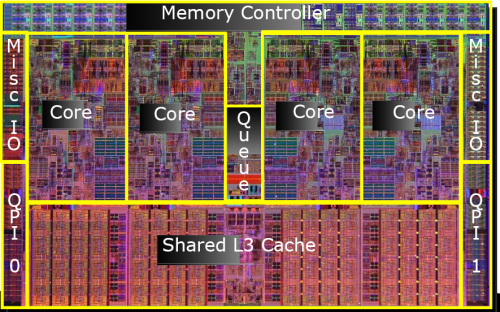
\includegraphics[width=0.45\textwidth]{cpu_diagram.png}
\caption{Quad-core Intel Core i7 CPU Architecture Diagram}
\label{fig:cpu_diagram}
\end{figure}

% [Use of GPUs – GPU Architecture]
Graphical Processing Units (GPU) are a newer technology than CPUs and serve a dedicated purpose of taking instructions from the CPU and performing multiple, hardware-based mathematical operations for translating three-dimensional shapes and coordinates into two-dimensional projections for rendering to a display, and runs multiple small programs called ``shaders” to handle colour and lighting. Due to the sheer amount of mathematical calculations that need to be performed to display something onto a display, GPUs are architected differently to a CPU. Modern graphics cards, such as NVIDIA’s Turing architecture, pictured in Figure \ref{fig:gpu_diagram}, are composed of multiple stream processors, each divided into hundreds of small cores which perform a single integer or floating-point operation. This stream processing approach allows for vast parallel computation over a large dataset in a paradigm called ``single instruction multiple data” (SIMD).

This parallelism was previously reserved for image and video processing but a few years ago NVIDIA released their CUDA API\cite{cuda_talk}\cite{CUDA} which allows developers to leverage the stream processing nature of the GPU for general-purpose computation. Scientific workloads from biomedical imaging\cite{luebke2008cuda} to deep learning\cite{tang2013deep} are now done on the GPU, and modern supercomputers, such as Summit, are built with large numbers of GPUs to accelerate workloads and perform previously-impossible simulations and workloads.

% \footnote{\url{https://devblogs.nvidia.com/nvidia-turing-architecture-in-depth/}}
\begin{figure}
\centering
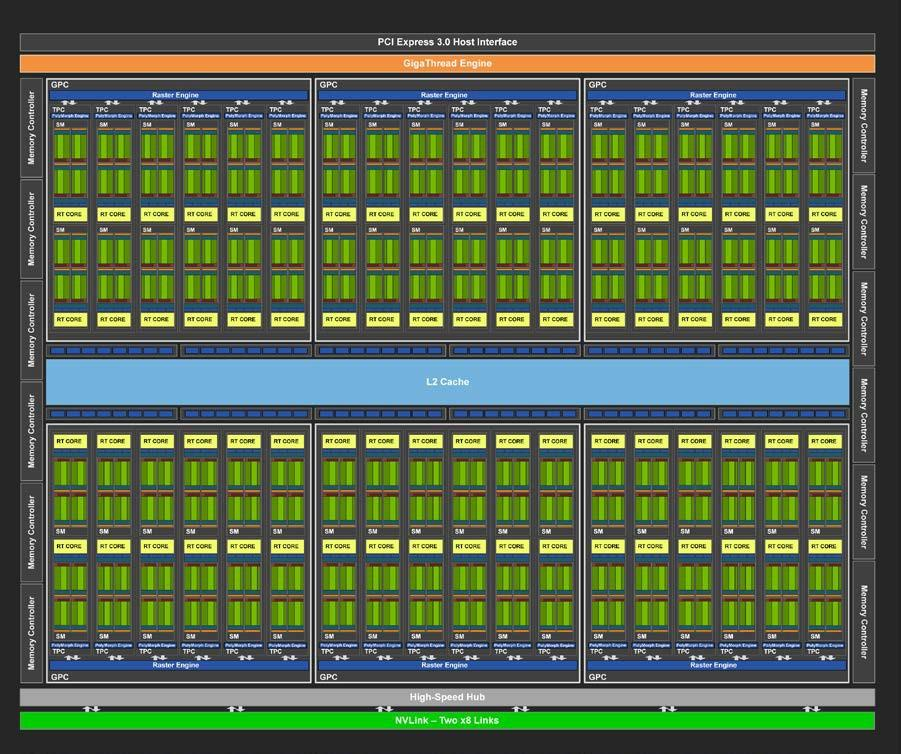
\includegraphics[width=0.45\textwidth]{gpu_diagram.jpg}
\caption{NVIDIA Turing GPU Streaming Multiprocessor Architecture Diagram}
\label{fig:gpu_diagram}
\end{figure}

% Miniapps
Mini-applications (``miniapp”) are a new area within the field of High Performance Computing (HPC). These applications are small, self-contained proxies for real applications (typically relating to simulation of physical phenomena) to quickly and concisely explore a parameter space, leading to focused and interesting performance results to investigate potential scaling and run-time issues or trade-offs\cite{miniapps}. Miniapps capture the behaviour and essence of their parent applications primarily because of two characteristics of many applications running on distributed systems: the performance of an application will mainly be constituted by the performance of a small subset of the code, and many of the physical models that constitute the rest of the application are mathematically distinct and generally have similar performance characteristics\cite{miniapps}.

\subsection{Objectives}

The SN (Discrete Ordinates) Application Proxy (SNAP) is a miniapp that acts as a proxy for discrete ordinates particle transport. It is modelled off another production simulation program developed by the Los Alamos National Laboratory called PARTISN, which solves the linear Boltzmann transport equation (TE)\footnote{Boltzmann Equation: \url{ https://en.wikipedia.org/wiki/Boltzmann_equation}}, simulating neutron criticality and time-independent neutron leakage problems\cite{partisn} in a multi-dimensional phase space. SNAP is a proxy to PARTISN because it provides a concise solution to a discretised, approximated version (though with no real-world relevance) of the same problem PARTISN solves, providing the same data layout, the same number of operations, and loads elements into arrays in approximately the same order.

The SNAP algorithm works by defining the phase space as seven dimensions: three in space (x, y, z), two in angle (octants, angles), one in energy (groups, or energy-based bins of particles), and one of time (time step). SNAP sweeps across the spatial mesh, starting in each of the octants proceeding towards the antipodal octant, performing a time-dependent calculation in each cell using information from the previous time-step and surrounding cells. This motion forms a wave-front motion that sweeps across the three-dimensional space from corner to corner, with work being divided along each diagonal for parallel execution

With this miniapp in mind, we define three key objectives that the project shall solve. Taken together, these will provide a holistic overview as to the validity and efficacy of this approach of converting CPU-bound parallelised algorithms to utilise the GPU instead (where appropriate). With the SNAP algorithm and open-source repository (specifically the C-based port of the code) in mind, the three objectives are:

\begin{itemize}

\item To instrument, profile, and analyse the current implementation of the code in order to identify areas of the code in which it would be applicable and beneficial to convert to CUDA-based parallelisation.

\item Using the identified areas found in problem 1, to fork the current C-based port of the SNAP GitHub repository\footnote{\url{https://github.com/lanl/SNAP}} and convert the candidate components and routines from OpenMP to utilise the CUDA libraries instead.

\item Following the reimplementation of the algorithm to CUDA technology, the last step is to analyse and evaluate the efficiency and efficacy of the new solution in comparison to the previous CPU-based approach. Ideally, a theoretical maximum efficiency of the approach will also be calculated mathematically, and the actual implementation compared against this as another measure of success.

\end{itemize}

%%%%%%%%%%%%%%%%%%%%%%%%%%%%%%%%%%%%%%%%%%

\section{Related Work}

A seminal work in the field of miniapps was written by Heroux et al\cite{miniapps}, defining the paradigm. Their Mantevo miniapp suite has show successful development of miniapps, such as MiniFE for finite element analysis and MiniMD for molecular dynamics simulations, to demonstrate their versatility and applicability. Others have demonstrated such success in other areas, such as Mallinson et al with ``CloverLeaf”\cite{mallinson2013cloverleaf}, and Los Alamos National Lab (\url{https://www.lanl.gov/projects/codesign/proxy-apps/lanl/index.php}). Miniapps have been shown to produce similar performance characteristics to their fully-fledged counterparts\cite{miniapps}, adding to the efficacy of the paradigm.

General-purpose simulations on GPUs have been studied for a long time, with GPUs being a core part of modern computing clusters\cite{debardeleben2013gpu}. Strong-scaling across multiple GPUs\cite{glaser2015strong} is the ideal approach. Consideration is taken also for conversion of existing codebases\cite{zhou2011gpu} and new, bespoke solutions designed with GPU architecture utilisation in mind\cite{glaser2015strong}. Bespoke solutions offer superior code architecture and speed, meaning calculation of theoretical maximum performance increase for a pre-existing code base will have to take this into account.

Writing GPU targeted miniapps in a developing area of work. Baker et al\cite{baker2012high} discuss implementation details of converting the KBA sweep algorithm of the Denovo code system to run on NVIDIA’s Titan GPU. Mallison et al\cite{mallinson2013cloverleaf} demonstrate too with CloverLeaf the performance advantages GPU-based architecture targeting can have over purely CPU-based versions. It is important to note that these performance increases might not necessarily be completely reflected in SNAP’s algorithm due to other considerations, such as the scaling characteristics of the algorithm\cite{shoukourian2014predicting} and communication technologies as highlighted by Glaser et al\cite{glaser2015strong}.

Performance of miniapps with respect to CPU- and GPU-based parallelisation frameworks have been explored previously and show promising results which add credence to the motivation of this project. Notably Martineau et al\cite{martineau2017productivity} reached the conclusion that compiling miniapps to CUDA resulted in greater efficiencies compared to other targets, though care is needed to consider the implementation (especially with respect to data accesses) to avoid the compiler introducing performance penalties.

Development of the solution must still mimic the behaviour of the original application however, so care must be taken to preserve this. Heroux et al\cite{miniapps} and Messer et al\cite{messer2015developing} outline the fundamental principles that a miniapp must adhere to and the considerations of forming a miniapp from the base application – all of which would help form testing criteria for this project and future projects to help preserve results and intrinsic behaviour.

%%%%%%%%%%%%%%%%%%%%%%%%%%%%%%%%%%%%%%%%%%

\section{Project Review}

In this section, we review the current progress made on the project so far and reflect upon how the project has progressed to this point, what has gone well and potential areas for improvement. A section follows discussing the plan for how the rest of the project will progress, outlining key stages, timeline and built-in contingency periods in order to complete the work.

\subsection{Current Progress}

The project has progressed well into the planning and design stage. Unfortunately, it is to be said that this is behind the schedule outlined in the project proposal and presentation given in May – a key item highlighted in the Reflection section that follows. Several key areas of consideration and development are underway, categorised as follows:

\begin{enumerate}
\item Setting up of a local development and testing environment
\item Developing a practical understanding of CUDA
\item Consolidation of the important facets of the algorithm into psuedocode
\item Development of a mathematical model for how the GPU-based version will operate under ideal conditions
\end{enumerate}


\subsubsection{Local Development and Testing Environment}

In order to maximise the value and amount of time that can be spent developing the project, it is crucial to develop it on a local, non-networked machine to avoid queueing for resources and latency with file transfers and the like.

A personal computer was allocated for the task because of its preferential components that can lend great speed and analytical power to the task. Its specifications are as follows:

\begin{itemize}
\item Intel® Core™ i7-6700K CPU, clock speed of 4GHz. It is a quad-core CPU with hyperthreading enabled for an apparent core count of 8.
\item NVIDIA GeForce GTX 1070 graphics card. Pascal architecture that supports the CUDA Compute functionality, 1.5Ghz base core clock, 8GB of GDDR5 memory, and 15 streaming multi-processors.
\item 16GB of DDR4 RAM
\end{itemize}

This will enable a good baseline assessment of how the SNAP program works on the system for a set of given inputs that can then be used for comparison to the GPU-based approach used on the same set of inputs.

For compilation of the code and to imitate a Linux-based computer cluster, Ubuntu will be used as the base operating system due to its wide-ranging support and package compatibility, in addition to having the following packages installed:

\begin{itemize}
\item Gnu C and C++ libraries – for compilation of C/C++ programs, as well as associated tooling such as \texttt{backtrace}.
\item \texttt{mpicc} to compile the standard C-port of SNAP
\item \texttt{OpenMP} to compile the standard C-port of SNAP
\item NVIDIA drivers and CUDA libraries
\item All supporting libraries that everything else depends upon
\end{itemize}

It was important for the program to be run as fast and ``as close to the metal” as possible to get accurate results from various executions because virtual machines or Docker containers could add unseen overheads and not give a true indication of speed or performance of the programs.

After the program has shown promising results (if any) on the local environment, it will be submitted to a computing cluster at the university and see if the solution scales with larger inputs. It’s possible that the program won’t show much improvement in the local environment as it could only marginally improve the performance, whereas it could scale up and save more time per calculation over a much larger input – the type of GPU the cluster runs and the relative amount of streaming multiprocessors in the GPUs versus the number of CPU cores/threads available has the potential to be a significant contributing factor to the results.


\subsubsection{CUDA Learning}

A core part of the progress made has been in learning and experimenting with the CUDA framework which is needed to execute the program on the GPU. It was covered at an introductory level as part of the CS402 High-Performance Computing module. From this, I independently explored the documentation and framework further with the aid of NVIDIA’s Developer Blog\footnote{\url{https://devblogs.nvidia.com/even-easier-introduction-cuda/}}, as well as harnessing additional resources online to gain a clear understanding of the technology.

With this knowledge in mind, as well as details about the architecture and layout of the graphics cards utilised in both the local and cluster environments the program is to be executed in, certain design implementations, such as data layout, quantity of data to transfer, and amount of blocks can be processed in parallel, can be confidently estimated and will guide the direction and effectiveness of the implementation.

\subsubsection{Mathematical Model}

In order to get a gist of the amount of reasonable work the GPU could handle at once and estimates for the amount of time and data movement needed for the optimal implementation, a mathematical model was developed to help visualise and describe the interactions between adjacent cells in the approximated algorithm that SNAP uses. The following assumptions were made when developing this model:

\begin{enumerate}

\item The algorithm defines the problem space as a three-dimensionality discretized grid of cells, each with their own values and interactions with their neighbouring adjacent cells – this forms the core of the SNAP algorithm (it itself approximating a continuous algorithm).

\item The problem space is cubic with side $ n $ for ease of modelling. A generalisation to a cuboidal space with dimensions $ (x, y, z) $ can be abstracted from the cubic model later.

\end{enumerate}

\begin{figure}
\centering
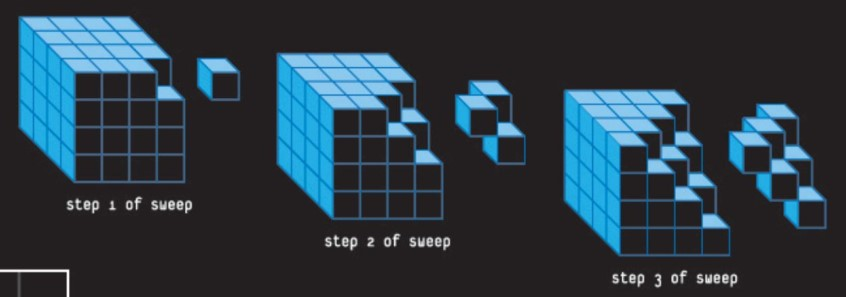
\includegraphics[width=0.45\textwidth]{Sweep.jpg}
\caption{Slices of a sweep of 3D grid}
\label{fig:3dsweepslice}
\end{figure}

Given these assumptions, we aim to derive the total number of communications between cells in the grid per iteration and how much work this equates to and how much can be parallelised at each stage.

There are $ 8 $ vertices of a cube so $ 8 $ octants to perform the sweep over. Each sweep is divided up into diagonal slices, shown in Figure \ref{fig:3dsweepslice}, of which there are $ (x + y + z) – 1 $ of them ($ 3n – 1 $ in this model). A key point to note is the dependency in each sweep of a slice on the slice before as the direction of the sweep is linear and calculations rely upon previous ones\footnote{As described in the documentation of the SNAP algorithm in their GitHub repository - \url{ https://github.com/lanl/SNAP/blob/master/docs/SNAP-overview-presentation-2015.pdf}}, and each combined sweep of all octants, after all results being collated, forms the basis of the next sweep.

The first $ n $ slices of the grid are comprised of the sum of the first $ n $ triangular numbers’ (i.e. $ 1, 3, 6, 10, 15… $)\footnote{Sequence A000217 in the ``On-line Encyclopedia of Integer Sequences'' (\url{https://oeis.org/A000217})}, worth of cells, with the final $ n $ slices having the same number also (just in reverse order). $ n - 2 $ slices exist between the 2 triangular-based pyramids formed from the previous step, allowing us to develop a function for the first $ m = n + \frac{n - 2}{2} $ slices, and mirror it to get the number of cells in any slice of the grid.

The number of cells in slice $ i $ of a cube of size $ n $ is thus given by the following formula:

\begin{equation}
cells(i) = \left\{
	\begin{array}{ll}
		tri(i) & \mbox{if } i \le n \\
		tri(i) - 3tri(i - n) & \mbox{if } i \le m \\
		cells(m - ((i - 1)\bmod m)) & \mbox{otherwise}
	\end{array}
\right.
\end{equation}

Where $ tri(i) $ represents the $i$th triangular number, $ 1 \le i \le 3n - 1 $. 

This means poor performance early on due to low numbers of cells per layer and the inter-slice dependency, but will ultimately scale well and to more graphics card given a large grid.

To work out data transfer, we need to figure out the amount of sends and receive actions are performed per slice. We can again work first out up to the first $ m $ slices, and take the mirror image for the rest of the slices, swapping the number of sends per slice for the receives of the mirror slice and vice versa. For the first $ n - 1 $ slices, each cell sends to 3 neighbouring adjacent cells in the next slice. When $ i \ge n $, we need to take into account the ``cut-off'' portions where some cells only send to 2 neighbours, hence:

\begin{equation}
sends(i) = \left\{
	\begin{array}{ll}
		tri(i) * 3 & \mbox{if } i < n \\
		(i\bmod(n - 1)) * 2 + \\
			(cells(i) - i\bmod(n - 1)) * 3 & \mbox{if } i \le m \\
		recvs(2n - i) & \mbox{otherwise}
	\end{array}
\right.
\end{equation}

The total number of receive actions is similar. The first cell has no neighbours to receive from, the second slice has only 1, the rest have three, then after the $n$th slice we need to consider where we only receive from 2 neighbours:

\begin{equation}
recvs(i) = \left\{
	\begin{array}{ll}
		0 & \mbox{if } i = 1 \\
		tri(i) & \mbox{if } i = 2 \\
		tri(i) * 3 & \mbox{if } i \le n \\
		(cells(i) - (2n - i)) * 3 & \mbox{if } i \le m \\
		sends(2n - i) \mbox{otherwise}
	\end{array}
\right.
\end{equation}

Both functions are defined in the domain $ 1 \le i \le 3n - 1 $.

If we let $ msg_s $ be the size of a message to send and $ msg_r $ the size of a message to receive from a neighbour (both in number of bytes), and knowing that the fastest data transfer rate of the PCI Express (PCIe) 2.0 bus connecting the graphics card and CPU together is 500MB/s\cite{PCIe}, we can calculate the time per slice to store data from the GPU as

\begin{equation}
time_s = \frac{sends(i) * msg_s}{5 \times 10^8}
\end{equation}

and to send data to it as

\begin{equation}
time_r = \frac{recvs(i) * msg_r}{5 \times 10^8}
\end{equation}

Aggregating these over all slices, alongside an assumed small, constant kernel function calculation time $ C $ over $ cells(i) $ cells in the slices, yields the best-case calculation time for the current approach. From here, we can interleave all 8 octants for calculation at once (of course managing the number of streaming multi-processors, which, after a point, we'd need to vastly scale hardware or queue work) to improve our throughput. $C$ ultimately depends on the type of graphics card being used.

\subsection{Reflection of Current Efforts}

Three areas come into focus when reviewing the current state of the project:

\subsubsection{Presentation}

Feedback from the presentation was positive, reinforcing and supporting the background research done earlier in the process. This gives me confidence going forward that the project will have a meaningful and relevant outcome to the field. The main issue highlighted with the project was the timeline I had originally set to do each stage of the project. When viewed in isolation, the timeline was generous and appropriate, but factoring in design decisions, examinations, and other deadlines, it became apparent that not enough contingency was built into the process for unseen eventualities and this has unfortunately resulted in the project being behind its original timeline. 

\subsubsection{Examinations}

One key reason was the error in not factoring in appropriate time for revision and examinations, which took up the bulk of May and early June, in which the project’s development faltered. This is a minor setback and a revised Gantt chart for future development is presented later in the report.
Development didn’t stop however, as the development environment was still established and, as part of the CS402 High-Performance Computing module, there was substantial headway made with regards to learning CUDA, architecting, and analysing parallelised programs. This knowledge stands me in good stead to progress the work back up to where it should be and at a more fundamentally sound level.


\subsubsection{Other}

Finally, an area that might need to be reviewed, even if just at a cursory level, is the Related Work section. The field of HPC is a fast moving one so, combined with NVIDIA’s announcement of their ``Super” consumer graphics cards\footnote{\url{https://www.nvidia.com/en-us/geforce/graphics-cards/rtx-2080-super/}} and other technologies, it would be beneficial to review the literature again to ensure that this project is still at the cutting-edge – if new papers and results have come to light, it can only help to bolster this project and the speed and effectiveness with which it can be produced.


%%%%%%%%%%%%%%%%%%%%%%%%%%%%%%%%%%%%%%%%%%

\section{Plan for Further Work}

Below is an itemised list, in order of what needs to be completed first, of the rest of the work needed to complete the project. The work spans all areas of conceptual design, development, testing, and reporting, due to the time impediments discussed in the reflection prior.

\begin{enumerate}

\item Exploring and confirming the mathematical model of the system to ensure that it’s representative of what is happening in the system, as well as ensuring it’s at least theoretically better than the current CPU-bound implementation.

\item Using the mathematical model as a guide for the ideal scenario, start to develop the CUDA-based alteration in earnest. Care being taken at this stage to write an appropriate kernel function and manage data transfer to be as minimal as possible.

\item Continually test the approach in a local testing environment that allows for parallelised C code to run on a CUDA-enabled device – ideally the bare-metal Linux environment setup on my personal machine but a VM with more than one CPU core allocated and GPU pass-through would suffice.

\item Once development has reached its final stages, collate a range of inputs for the program (provided in the original SNAP repository) and execute them both with the old SNAP code and the new GPU-accelerated program.

\item Compare and contrast the results of step 4, making any necessary design tweaks or fixes to the implementation as required.

\item Fully document the findings in the final dissertation, alongside the methodology, details of the design, and implementation nuances or difficulties faced.

\end{enumerate}


\subsection{Project Management}

The code for the project will be managed by a public code repository hosted on GitHub at the following address: \url{https://github.com/alshort/SNAP}. It will be hosted under the same licence at the original and follow the usual best practices with regards to version control of atomic changes and experimental items done on a new branch and merged down to master if successful. Version control will keep a backup of different stages of the code should reversion be required. It will also be open-source allowing others to contribute to it in the future.

Finally, the project will be managed at a higher-level by producing work in-line with the revised timeline (as seen below), in addition to frequent communication with the project supervisor and any additional people as required to help provide solutions to impediments, feedback on current progress and the overarching approach, and for further advice should it be needed at any stage of the project.

The Gantt chart of the rest of the timeline of the project is as follows:

\begin{figure}[h!]
\centering
\ganttset{calendar week text=\small{\startday}}
\begin{ganttchart}[
    hgrid,x unit=0.08cm,
    hgrid style/.style={draw=black!5, line width=.75pt},
    vgrid={draw=none,draw=none},
    bar label node/.style={text width=2cm,align=right,font=\scriptsize\RaggedLeft,anchor=east},
    group label node/.style={text width=2cm,align=right,font=\bf\scriptsize\RaggedLeft,anchor=east},
    time slot format=little-endian]{01-07-2019}{12-09-2019}
\gantttitlecalendar{month=shortname, week=4} \\
\ganttgroup{Total Duration}{01-07-2019}{12-09-19}\\
% Investigation and Design
\ganttgroup{Investigation and Design}{01-07-19}{31-07-19}\\
\ganttbar{Collating Stacktraces and Data}{01-07-19}{20-07-19}\\
\ganttbar{Mathematical Model}{01-07-19}{27-07-19}\\
\ganttbar{Finalise CUDA Education}{01-07-19}{31-07-19}\\
% Design and implementation
\ganttgroup{Design and Implementation}{01-07-19}{30-08-19}\\
% Testing
\ganttgroup{Testing}{15-07-19}{14-08-19}\\
\ganttbar{Local Profiling and Benchmarking}{15-07-19}{14-08-19}\\
\ganttbar{Cluster Profiling and Benchmarking}{14-07-19}{14-08-19}\\
% Dissertation
\ganttgroup{Dissertation}{26-08-19}{12-09-19}\\
\ganttbar{Writing}{26-08-19}{10-09-19}\\
\ganttbar{Proof Reading and Editing}{5-09-19}{12-09-19}
\end{ganttchart}
\end{figure}


%%%%%%%%%%%%%%%%%%%%%%%%%%%%%%%%%%%%%%%%%%



% Research approach/methodology, etc...
% \section{Research Processes}

% The research methodologies utilised in this project can be categorised into two stages.

% The first stage is for the research undertaken as part of this proposal to assess the academic field relating to high-performance computing and GPU-based parallelisation. The Library at University of Warwick offers a collection of databases of scholarly content (articles, journals, data etc.) for students to search through. These databases are trusted, informative sources of research – from IEEE to ACM – that allows for search by keywords and phrases. Using a handful of seminal papers that are central to the HPC and miniapp fields, searches were done relating to these terms, and citations from previous papers followed, to accumulate varied and relevant research to ascertain the current state-of-the-art, theories, proof-of-concepts, and existing work. This is in aid of cementing and consolidating knowledge of the field, identifying key analytical techniques and metrics to suitably measure and evaluate the final output of the project (especially against existing systems) and to identify gaps in the literature that this project ultimately aims to contribute to.

% The other stage is for the methodology with which the project will be undertaken. Principally with regards to how the initial analyses and performance profiling of the SNAP project will be done and how the modified project will be tested and assessed.

% In terms of the analysis and profiling of the code in its current state, a swathe of programs and modifications will be performed in order to fully understand the time each section of the code takes to run and how the OpenMP library parallelises the code (this last stage is in conjunction with a manual inspection of the code as well as flow-charting key aspects of the algorithm). From this, a well-defined theoretical understanding will be ascertained that would allow us to derive a more granular model of parallelisation to use on the critical areas of the codebase to allow for our GPU-based model to be most effective.

% Testing the final solution will be performed in comparison to the current codebase ideally on different host machines. Running both applications, with the same input data and controlling as many external variables as possible (such as keeping the amount of background processes consistent, performing multiple runs to calculate an average etc.), on a consumer-focused target machine with a multicore CPU and dedicated GPU will provide an initial result to show if the modifications produce the desired speed increase. From this, it is hoped to conduct further research into the efficacy of the solution by running the program on University of Warwick’s Tinis or Orac computing clusters. Execution on a cluster will demonstrate, if any, the scalability of the solution, and if there is any difference between running on highly multicore CPUs (several Intel Xeon processors) and running on several compute-specific GPU cards (NVIDIA P100 or Tesla K68 GPUs, for example).

% Our research will conclude by compiling, contrasting, and comparing the performance characteristics of both applications to gauge the superior software architecture for SNAP, and from this, hope to learn about the advantages and disadvantages of GPU-based miniapps.


% Timeline, constraints, risk, etc...
% \section{Project Management}

% \subsection{Management and Accountability}

% For the project to progress, it is important that consistent work is made and is made in the right direction. The code for the project will be uploaded to a public-facing GitHub repository to keep track of the progress of the project, in addition to being able to properly source control the software to allow for experimental branches, backing up of code, and to manage future releases.

% Communication with the supervisor for this project will be done on a weekly basis via email, Skype, or in-person meetings to discuss the progress of the previous week, demonstrate current findings or developments, and to deliberate next steps.

% The final write-up for this project will be done in a pipelined fashion, wherein different sections and aspects of the dissertation are written whilst others are submitted to the supervisor for consideration and approval for accuracy and readability.

% \subsection{Timeline}

% An estimated timeline of the project follows overleaf.

%\newgeometry{vmargin=1cm, hmargin=1cm}
%\begin{landscape}
%\thispagestyle{empty}\centering
%
%\ganttset{calendar week text=\small{\startday}}
%\begin{ganttchart}[
%    hgrid,x unit=0.1cm,
%    hgrid style/.style={draw=black!5, line width=.75pt},
%    vgrid={draw=none,draw=none},
%    bar label node/.style={text width=3cm,align=right,font=\scriptsize\RaggedLeft,anchor=east},
%    group label node/.style={text width=3cm,align=right,font=\bf\scriptsize\RaggedLeft,anchor=east},
%    time slot format=little-endian]{18-02-2019}{30-09-2019}
%\gantttitlecalendar{month=shortname, week=4} \\
%\ganttgroup{Total Duration}{18-02-19}{30-09-19}\\
%% Investigation and Design
%\ganttgroup{Investigation and Design}{21-02-19}{08-04-19}\\
%\ganttbar{Initial Investigation}{21-02-19}{05-03-19}\\
%\ganttbar{In-depth Profiling and Analysis}{24-02-19}{03-04-19}\\
%\ganttbar{Researching Libraries and Techniques}{28-03-19}{08-04-19}\\
%% Design and implementation
%\ganttgroup{Design and Implementation}{25-03-19}{30-06-19}\\
%\ganttbar{Initial Design}{25-03-19}{30-04-19}\\
%\ganttbar{Programming}{22-04-19}{30-06-19}\\
%% Testing
%\ganttgroup{Testing}{15-05-19}{14-07-19}\\
%\ganttbar{Local Profiling and Benchmarking}{15-05-19}{14-06-19}\\
%\ganttbar{Cluster Profiling and Benchmarking}{14-06-19}{14-07-19}\\
%% Dissertation
%\ganttgroup{Dissertation}{17-06-19}{30-09-19}\\
%\ganttbar{Writing}{17-06-19}{17-09-19}\\
%\ganttbar{Proof Reading and Editing}{01-09-19}{30-09-19}
%\end{ganttchart}
%\end{landscape}
%\newgeometry{vmargin=2.25cm, hmargin=2.25cm}

% Overview of progress, etc...
% \section{Progress}

% Currently, the field of high-performance computing with respect to GPU-based parallelisation workloads has been initially researched (see the ``Related Work” section above). From this, several considerations regarding the profiling and benchmarking process of analysing the SNAP project to identify easily GPU-parallelisable workloads has been developed and will guide the design stage of the project and the likely implementation that will result.

% An investigation into the pipeline and API of NVIDIA’s CUDA technologies has been started also. It is important to fully understand the central tenants and paradigms of a technology before any implementation that aims to use it can get underway. This stage will progress smoothly because of NVIDIA’s dominance in the market place, the age and maturity of the technology, and its prevalence in HPC applications.

% Finally, a clone of the SNAP GitHub repository has been downloaded and study of the provided documentation and algorithm (from the C-based port of the code, which is what this project will focus on) has begun. The next stage in this process is to choose the appropriate running environment for the application, to start and successfully execute the application with a sample workload, and to begin instrumentation and profiling of the code.

% Summary, future work, etc...
% \section{Conclusion}
% Whilst the aim of this research proposal is to ascertain the potential performance increases of converting the SNAP miniapp to run on a GPU-based architecture, it also highlights the opportunity to formalise and contribute towards different aspects of the miniapp field that have been explored but not yet fully developed.

% Introduction of new or use of existing software profiling and diagnostic techniques will be used to identify areas of the codebase that have the potential for increased parallelism – potentially the basis for an automated system to translate serial or partially-parallel code to fully parallel for the most applicable available architectures. Development and testing of the implementation will follow, which will hopefully lead to a successful, open-source reimplementation of the SNAP algorithm, and ideally produce recommendations for parallelising certain components or algorithms based on data structures, algorithm design, or strong or weak scaling characteristics of certain parts of a code base.

% The research proposal finally outlines the direction of the project and the current progress made.

% \nocite{*}

\bibliographystyle{unsrt}
\bibliography{interim_report}

\end{document}